\documentclass[12pt]{article}
\usepackage[utf8]{inputenc}
\usepackage[english, main=bulgarian]{babel}
\usepackage{hyperref}
\usepackage{url}
\usepackage{graphicx}
\usepackage{geometry}
\geometry{left=3cm,right=1cm,top=1cm,bottom=3cm}
\usepackage{xcolor}
\usepackage{tikz}
\usetikzlibrary{trees}
\usepackage{tabularx}
\hypersetup{
	colorlinks,
	linkcolor={black},
	citecolor={black},
	urlcolor={black}
}

\begin{document}
	
\includegraphics[width=0.9\textwidth]{logo.png} \\
	\selectlanguage{bulgarian}
	\begin{center}
		\textbf{СЕДЕМНАДЕСЕТА УЧЕНИЧЕСКА КОНФЕРЕНЦИЯ \\ УК’17} \\ \vspace{3cm}
		\textbf{ТЕМА НА ПРОЕКТА}\\
		\large{Система за управление на обучението}\\ \vspace{3cm}
		\textbf{Автори:}\\
		Алекс Иванов Цветанов (8-ми клас) \\ и \\ Димо Димов Чанев (9-ти клас)\\
		СМГ, София\\ \vspace{3cm}
		
		\textbf{Научени ръководители (консултанти):} \\
		Красен Фердинандов и Васил Тинчев
	\end{center}
	
	\newpage
	\tableofcontents
	\newpage
	\begin{abstract}
		\large{
			Факт е, че има създадени вече системи за управление на обученията. Те имат някои недостатъци. Например: видеата на уроците са с продължителност 3-4 часа - твърде много; повечето системи нямат практически задачи за упражнение (програмиране се учи най-добре с практика, която липсва); други системи имат само теоретични тестове (напълно достатъчно за добро усвояване на знанията), но така не се отчитат практическите умения.
			
			Идеята на нашия проект е да направим онлайн система за управление на обученията, която да съчетава добри практики при организиране на уроците, така че да е интересно, полезно и максимално улеснено за обучаващия се. Най-важната част на проекта ни е да стимулираме бъдещия програмист, като му покажем, че не е толкова трудно, колкото звучи. Това става чрез онлайн състезания, насочени към неговото ниво, със сертификати и награди за най-добрите.
			
			Проектът ни е предназначен главно за начинаещи и по-напреднали в програмирането. Състезанията ще съдържат теоретична част, но най-вече ще бъдат ориентиране към практиката.
			
			Системата за теставане на практическите задачи е „\foreignlanguage{english}{The Judgata}“, отделен проект, който ние интегрираме в нашия.
			
			В този проект се включват и нашите преподаватели Делян Пирински, Краси Паскалев, Красен Фердинандов и Васил Тинчев.
		}
	\end{abstract}
	\newpage
	\section{Увод}
	Нашия проект представлява онлайн система за управление на обученията, която да съчетава най-добрите практики при организиране на уроците, така че да е интересно, полезно и максимално улеснено за обучаващия се. Най-важното в проекта ни е да поощряваме бъдещия програмист, като му демонстрираме, че не е толкова трудно, колкото звучи. Това става чрез онлайн състезания, насочени към неговото ниво, със сертификати и награди за най-добрите. \\
	\\
	Проектът ни е предназначен за начинаещи и по-напреднали в програмирането. Състезанията ще съдържат теоретична част, но най-вече ще бъдат ориентирани към практиката. \\
	\\
	Системата за теставане на практическите задачи е „\foreignlanguage{english}{The Judgata}“, отделен проект, който ние интегрираме в нашия. \\\vspace{0.5cm}
	
	
\includegraphics[width=0.9\textwidth]{chat} \\
	\newpage
	\section{Описание на реализацията}
	Схемата по-долу демонстира отделните части на приложението и връзките между тях:\\ \vspace{0.5cm} \\
	\tikzstyle{every node}=[draw=black,thick,anchor=west]
	\tikzstyle{selected}=[draw=red,fill=red!30]
	\tikzstyle{selectedg}=[draw=green,fill=green!30]
	\tikzstyle{selectedo}=[draw=orange,fill=orange!30]
	\tikzstyle{selectedb}=[draw=blue,fill=blue!30]
	\tikzstyle{optional}=[dashed,fill=gray!50]
	\begin{tikzpicture}[%
	grow via three points={one child at (0.5,-0.7) and
		two children at (0.5,-0.7) and (0.5,-1.4)},
	edge from parent path={(\tikzparentnode.south) |- (\tikzchildnode.west)}]
	\node {Приложение}	
	child { node {Ученическа система}
		child { node {Статична част}
			child { node {Секция „Курсове“}}
			child { node {Секция „Видео уроци“}}
			child { node {Секция „Презентации“}}
		}
		child [missing] {}				
		child [missing] {}				
		child [missing] {}
		child { node {База данни}}
		child { node {Сертификати}}
	}
	child [missing] {}				
	child [missing] {}				
	child [missing] {}
	child [missing] {}				
	child [missing] {}				
	child [missing] {}
	child { node {Тестваща система - The Jugdata}
		child { node {База данни}}
		child { node {Външен вид}}
	}
	child [missing] {}				
	child [missing] {}	
	child { node {Чат/Форум}
		child { node {База данни}}
		child { node {Стаи}}
	}
	;
	\end{tikzpicture}
	\\\vspace {1cm} \\
	{\centering 
\includegraphics[width=0.65\textwidth]{cert}}
	\newpage
	\section{Избор на програмно-технически средства}
	Технологиите, които използваме са добре известни и са се доказали с времето. Те са:
	\begin{itemize}
		\item \foreignlanguage{english}{NGINX} сървър
		\item \textcolor{green!60!black}{\foreignlanguage{english}{Node.JS \& MongoDB} (\foreignlanguage{english}{The Judgata})}
		\item \textcolor{blue}{\foreignlanguage{english}{JADE} (\foreignlanguage{english}{The Judgata})}
		\item \textcolor{black}{\foreignlanguage{english}{Reveal.JS} - инструмент за създаване на презентации}
		\item \textcolor{orange}{\foreignlanguage{english}{Bootstrap (Jumbotron)}}
		\item \textcolor{red}{\foreignlanguage{english}{FastCGI - Fast Common Gateway Interface, C++, MySQL} (ученическа система)}
	\end{itemize}
	\vspace{0.5cm}
	На \foreignlanguage{bulgarian}{с}хемата по-долу виждате отделните  части на приложението заедно със съответната технология:\\
	\vspace{0.25cm} \\
		\begin{tikzpicture}[%
		grow via three points={one child at (0.5,-0.7) and
			two children at (0.5,-0.7) and (0.5,-1.4)},
		edge from parent path={(\tikzparentnode.south) |- (\tikzchildnode.west)}]
		\node[selected] {NGINX сървър}	
		child { node {Приложение}
			child { node {Ученическа система}
				child { node {Статична част}
					child {
						node[selectedo] {Bootstrap (Jumbotron)}
						child { node {Секция „Курсове“}}
						child { node {Секция „Видео уроци“}}
					}
					child [missing] {}				
					child [missing] {}	
					child { 
						node[selected] {Reveal.JS}
						child {
							node {Секция „Презентации“}
						}
					}
				}
				child [missing] {}	
				child [missing] {}				
				child [missing] {}				
				child [missing] {}				
				child [missing] {}	
				child { node {База данни}
					child { node[selected] {MySQL}}
				}			
			child [missing] {}	
				child { node {Сертификати}}
			}
			child [missing] {}			
			child [missing] {}					
			child [missing] {}	
			child [missing] {}				
			child [missing] {}				
			child [missing] {}
			child [missing] {}				
			child [missing] {}				
			child [missing] {}
			child { node {Тестваща система - The Jugdata}
				child { node {База данни}
					child { node[selectedg] {MongoDB}}
				}
				child [missing] {}
				child { node {Външен вид}
					child { node[selectedb] {JADE}}
				}
			}
			child [missing] {}				
			child [missing] {}
			child [missing] {}				
			child [missing] {}	
			child { node {Чат/Форум}
				child { node[selectedg] {Node.JS}
					child { node {База данни}
						child { node[selectedg] {MongoDB}}
					}			
					child [missing] {}	
					child { node {Стаи}}
				}
			}
		}
		;
	\end{tikzpicture}
	\newpage
	\section{Описание на програмната система/програмното осигуряване} 
	Тъй като в проекта ни се налага дя работим с пароли за потребителите, използваме някой алгоритми за хеширане. \\ \vspace {0.5cm}
	%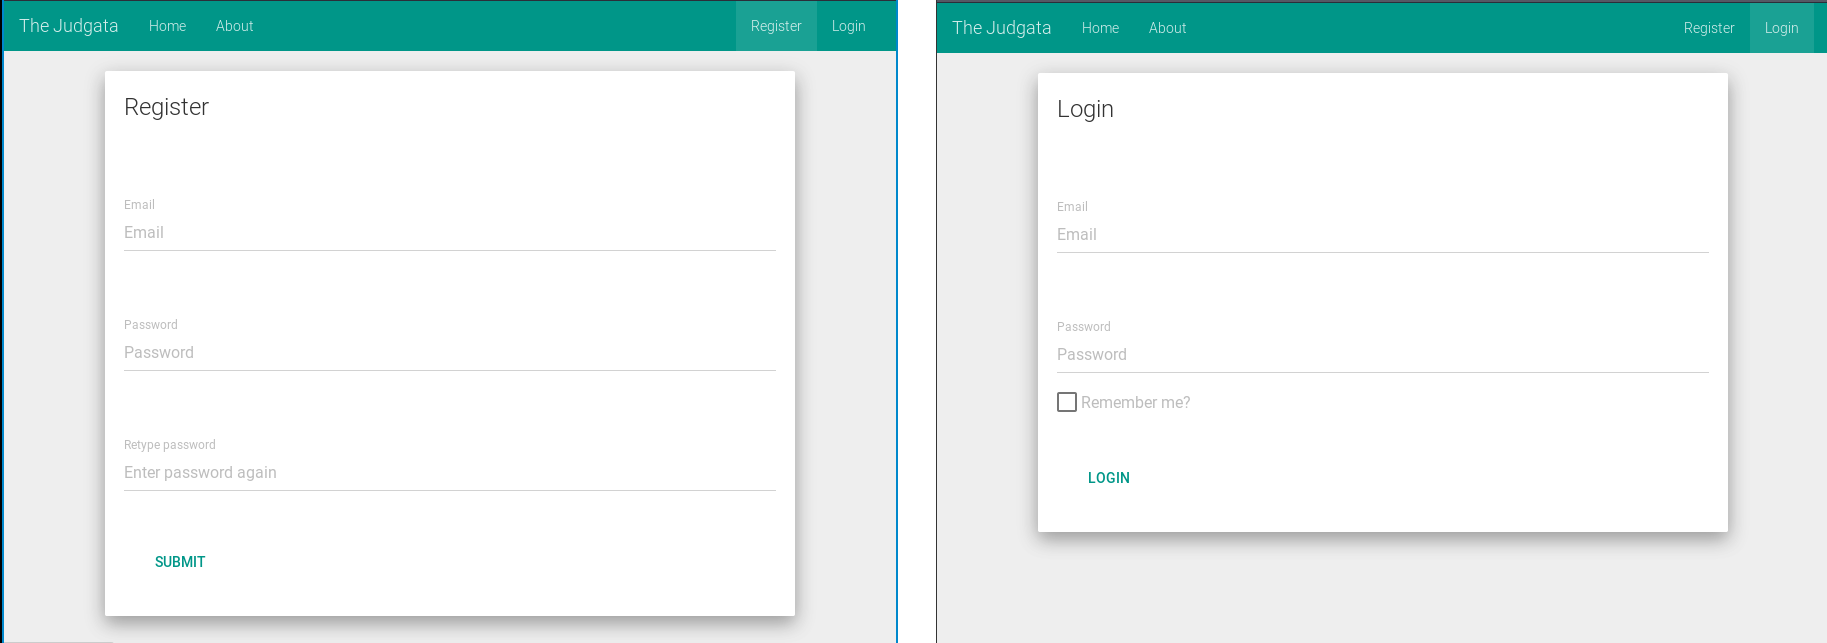
\includegraphics[width=1\textwidth]{logandreg} \\ \vspace {0.5cm}
	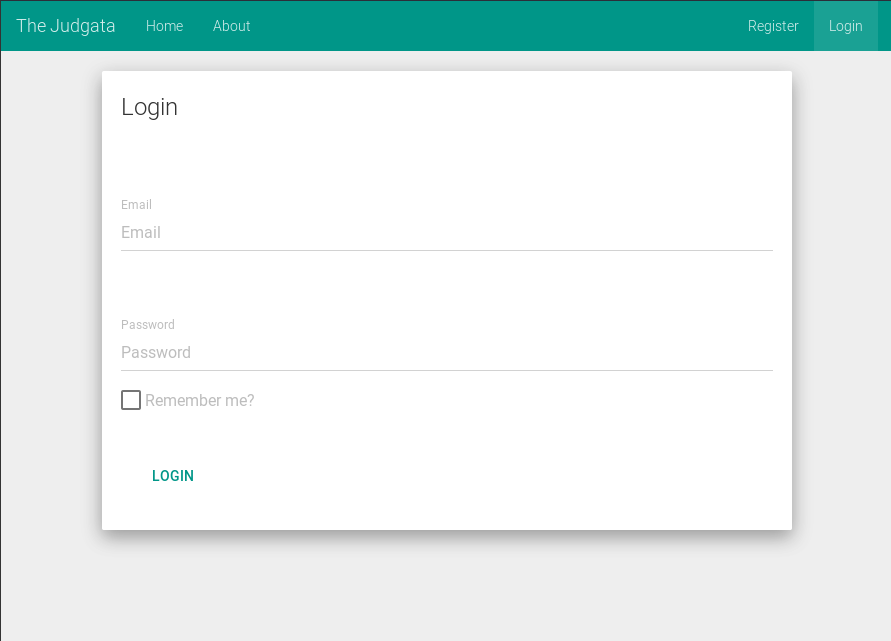
\includegraphics[width=0.80\textwidth]{login} \\ \vspace {0.5cm}
	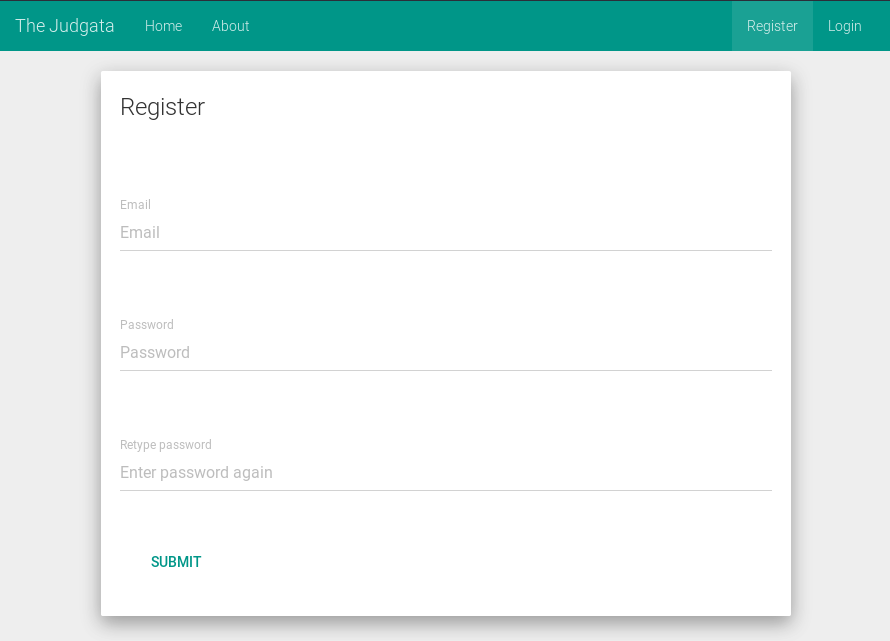
\includegraphics[width=0.80\textwidth]{register}
	\newpage
	\section{Защо този проект е по-добър от вече създадени такива?}
	\begin{table}[ht]
		\centering
		\resizebox{\textwidth}{!}
		{
			\begin{tabular}{c|c|c|c}
				& \foreignlanguage{english}{Telerik Academy by Progress} & Уча.се & Този проект\\
				\hline
				& & &\\
				Продължителност & & & \\ 
				на & 3-4 часа & 3-4-5 минути & 10-12-15 минути \\ 
				един урок & & &\\
				& & &\\
				\hline
				& & &\\
				Практически задачи & Да & Не & Да \\ 
				& & &\\
				\hline
				& & &\\
				Теоретични задачи & Да & Да & Да \\ 
				& & &\\
				\hline
				& & &\\
				Безплатни ресурси & Не и теоретичните задачи & Не & Да \\ 
				& & &\\
				\hline
				& & &\\
				Издаване на сертификати & Да & Не & Да \\
				& & &\\
				\hline
				& & &\\
				Възможност за & & & \\ 
				индивидуална работа с & Не & Не & Да \\
				обучаващия се & & &\\ 
				& & &\\
				\hline
				
				
			\end{tabular}
		}
	\end{table}
	\newpage
	\section{Изложение}
	Нашия проект представлява онлайн система за управление на обученията, която да съчетава най-добрите практики при организиране на уроците, така че да е интересно, полезно и максимално улеснено за обучаващия се. Най-важното в проекта ни е да поощряваме бъдещия програмист, като му демонстрираме, че не е толкова трудно, колкото звучи. Това става чрез онлайн състезания, насочени към неговото ниво, със сертификати и награди за най-добрите. \\\vspace {3cm} \\
	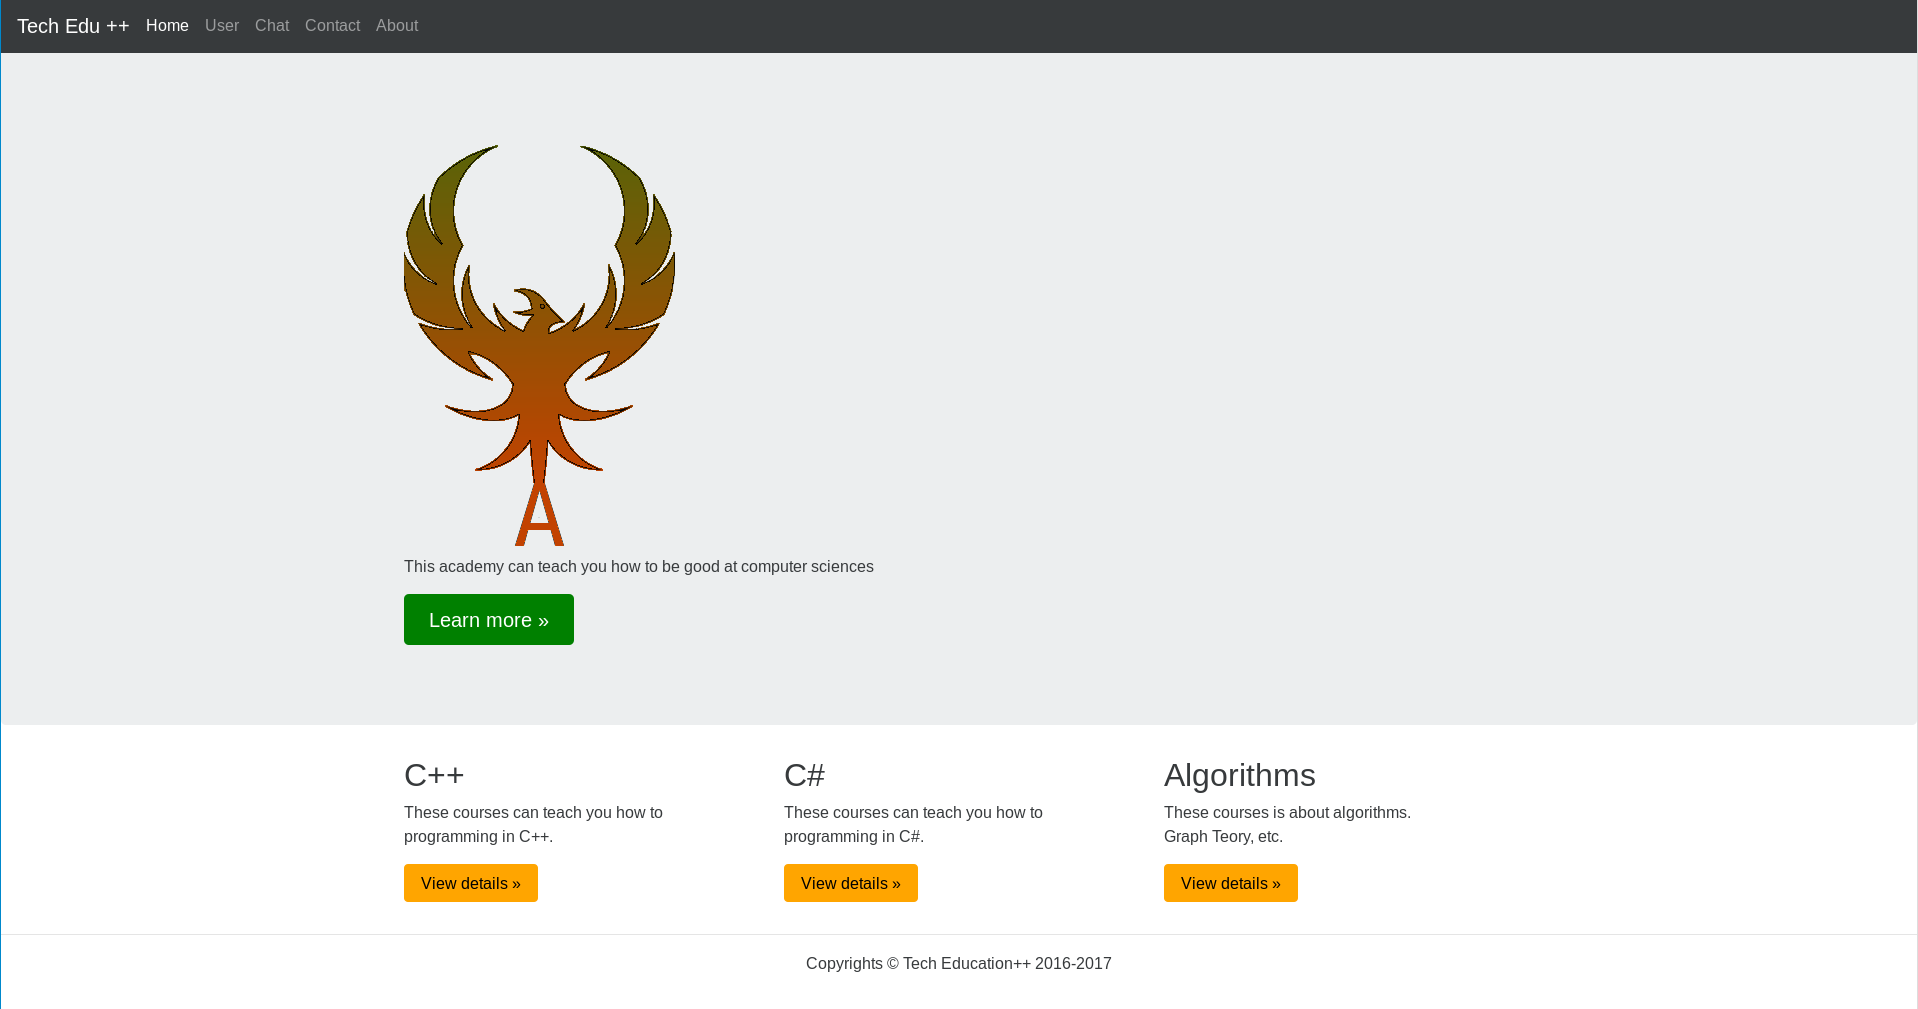
\includegraphics[width=0.9\textwidth]{academy} \\
	\section{\underline{\href{https://infocourse.techedu.cf}{Преглед на проекта}}}
	\section{\underline{\href{https://judge.techedu.cf}{Преглед на The Judgata}}}
	\newpage
	\section{Благодарности}
	Специални благодарности на:
	\begin{itemize}
		\item Мария-Йоанна Александрова за добрите идеи по отношение на дизайна
	\end{itemize}
	Благодарности също за:
	\begin{itemize}
		\item УчИМИ - Ученически Институт по Математика и Информатика
		\item БАН - Българска Академия на Науките
		\item СМГ - Софийска Математическа Гимназия
	\end{itemize}
	\selectlanguage{english}
	\begin{thebibliography}{9}
		\bibitem{reaveal}
		{Reveal.JS}.
		{http://lab.hakim.se/reveal-js/}. \\
		Copyright $\copyright\;$ 2016 Hakim El Hattab. All rights reserved.
		\bibitem{judgata}
		{The Judgata}.
		{https://judge.techedu.cf/}. \\
		Copyright $\copyright\;$ 2007 Free Software Foundation, Inc. All rights reserved.
		\bibitem{dom-to-image}
		{DOM to image}.
		{https://github.com/tsayen/dom-to-image}. \\
		Copyright $\copyright\;$ 2015 Anatolii Saienko
		\bibitem{letschat}
		{Let's chat}.
		{https://github.com/sdelements/lets-chat}. \\
		Copyright $\copyright\;$ 2012-2015 Houssam Haidar
		\bibitem{latex}
		{\LaTeX}.
		{https://www.latex-project.org/}.
	\end{thebibliography}
\end{document}